\chapter{Contagem aproximada}
\label{chap:morris}


\section{O Problema}

O problema da \textbf{contagem aproximada} consiste em contar um grande número de elementos usando pouca memória.  
Esse problema foi abordado pela primeira vez por Robert  Morris no artigo ~\citep{morris:78}, 
em que o autor descreve a tentativa de se contar eventos cujas frequências podiam chegar até 130 mil, mas usando apenas contadores de 8 bits.

Um registrador de $n$ bits pode armazenar inteiros entre $0$ e $2^n-1$. 
Dessa forma, em um computador que possui registradores de 8 bits, pode-se contar até 255.
Assim, Morris projetou um algoritmo para armazenar contagens \textit{aproximadas}, 
uma vez que, não era possível manter as frequências \textit{exatas} dos eventos em sua máquina.

\section{Algoritmo de Morris}

Para se armazenar \textit{exatamente} um valor entre $0$ e $n$, são necessários registradores com $\Omega(\lg n)$ bits. 
Então, para que seja possível contar o número de elementos em um conjunto com até $n$ elementos usando menos bits, 
deve-se abandonar a \textit{exatidão} da contagem e buscar alternativas aceitáveis.

Uma das primeiras ideias é manter o valor de $\lg n$ ao invés de $n$. 
Neste caso, se $X$ fosse o valor armazenado em um contador, $2^X$ seria utilizado como estimador \textit{aproximado} de $n$.
Para isto, seriam utilizados $O(\lg \lg n)$ bits.
Dessa forma, a política de incremento desse contador passa a ser a questão central.
Morris propôs um método probabilístico para resolver esse incremento.

Morris sugeriu originalmente utilizar um contador $X$ para armazenar a contagem do número de elementos em um dado conjunto $\Mbb$.
A cada novo elemento examinado de $\Mbb$, o contador $X$ seria incrementado com probabilidade $2^{-X}$.
Assim, o valor $2^{X} - 1$ passaria a ser adotado como a estimativa do total de elementos, 
sendo que o $-1$ é para que essa aproximação se ajustasse à situação em que não houvessem itens, ou seja, $\Mbb = \emptyset$.

A versão da estratégia de Morris que pode ser vista no Algoritmo \ref{prog:morris}
é baseada em uma ideia da seção \textit{Algorithm} do artigo ~\citetitle*{ApproximateCountingAlgorithm}~\citep{ApproximateCountingAlgorithm}.
Essa versão expressa a condição de incremento do contador como um experimento de lançamento de moedas. 
Sempre que um novo elemento do conjunto $\Mbb$ é examinado, o lançamento de $X$ moedas é simulado. 
O contador é incrementado somente quando os resultados de todos os lançamentos forem cara.
E a probabilidade deste evento ocorrer é $2^{-X}$. Na prática, para mimetizar o jogar de moedas, 
um número aleatório $r$ de $X$ bits é gerado, e $X$ é incrementado apenas se $r = 0$.

Segue o pseudocódigo:
\begin{programruledcaption}{
Algoritmo de Morris\label{prog:morris}
\\ \textbf{Entrada:} conjunto $\Mbb$
\\ \textbf{Saída:} estimativa de $|\Mbb|$
\label{prog:flajolet-martin}
}
  \begin{lstlisting}[
    language={[brazilian]pseudocode},
    style=pseudocode,
    style=wider,
    functions={},
    specialidentifiers={},
    deletekeywords={de}
  ]
      funcao Morris($\Mbb$) 
        X := 0
        para cada elemento de $\Mbb$ \kw{faça}
          faça o lançamento de X moedas
          se X = 0 ou os resultados de todos os lançamentos forem cara \kw{faça}
            X := X + 1
          fim
        fim
        devolva $2^X - 1$
      fim
  \end{lstlisting}
\end{programruledcaption}

\section{Análise da aproximação}
\label{sec:morris:analysis}

Esta seção busca esclarecer o quanto a estimativa do Algoritmo \ref{prog:morris} se distância do tamanho real do conjunto $\Mbb$ dado. As provas
serão baseadas nas notas de aula de \citep{LectureNotesAndoni}.

Considere que $2^{X_n} - 1$ é a estimativa devolvida pela função Morris($\Mbb$) tendo como entrada um conjunto $\Mbb$ com $n$ elementos.
Neste caso, $X_n$ é o valor do contador $X$ antes do término da execução da função.
Evidentemente, $X_n$ é uma variável aleatória que depende de $n$ e dos resultados dos lançamentos de moedas feitos durante a execução do algoritmo.
Dessa forma, $2^{X_n} - 1$ é também uma variável aleatória.

Agora, determinar $\Ebb[2^{X_n} - 1]$ passa a ser a questão central.

Para $n = 0$, $X_0 = 0$ e portanto,
\[ \Ebb[2^{X_0} - 1] = \Ebb[2^0 - 1] = E[0] = 0 \ .\]

Para $n = 1$, $X_1 = 1$ devido à condição $X = 0$ na linha $5$ da função \ref{prog:morris}. E assim, 
\[ \Ebb[2^{X_1} - 1] = \Ebb[2^1 - 1] = E[1] = 1 \ .\]

A determinação de $E[2^{X_3} - 1]$ está ilustrada na árvore da Figura \ref{fig:morris-tree}.
Nessa árvore, encontram-se os possíveis resultados do contador $X$ durantes as iterações da função de Morris.
A setas da cor verde indicam que o contador foi incrementado e as da cor vermelha, que o contador permaneceu com o mesmo valor.

\begin{figure}
  \centering
  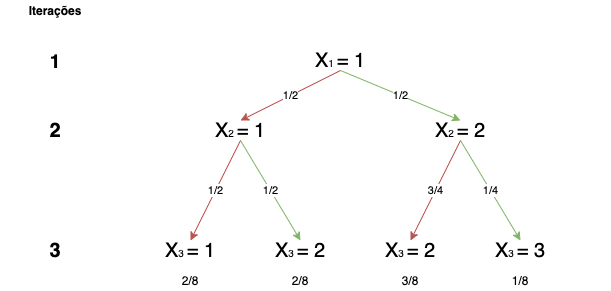
\includegraphics[scale=0.50]{figuras/morris-tree.png}
	\caption{Árvore de decisão para quando $|\Mbb| = 3$ no Algoritmo \ref{prog:morris}}\label{fig:morris-tree}
\end{figure}

Segue que
\begin{align*}
  \Ebb[2^{X_3} - 1] 
    &= \frac{2}{8} \Big(2^1 - 1\Big) + \frac{2}{8} \Big(2^2 - 1\Big) + \frac{3}{8}\Big(2^2 - 1\Big) + \frac{1}{8} \Big(2^3 - 1\Big) \\
    &= \frac{2}{8} \Big(1\Big) + \frac{2}{8} \Big(3\Big) + \frac{3}{8} \Big(3\Big) + \frac{1}{8} \Big(7\Big) \\
    &= \frac{24}{8} \\
    &= 3 \ .
\end{align*}

Em todos os exemplos calculados, $\Ebb[2^{X_n} - 1] = n$. O Lema a seguir mostra que isso não é coincidência.


\begin{lemma} \label{morris:expected_value}
A estimativa do Algoritmo \ref{prog:morris} é não-viesada, ou seja, $\Ebb[2^{X_n} - 1] = n$.
\end{lemma}

\begin{proof}
A prova será por indução em $n$. 

Para $n = 0$, $X_n$ = 0. Logo, $\Ebb[2^0 - 1] = 0$.

Suponha que para $n > 0$, $\Ebb[2^{X_{n-1}} - 1] = n-1$.

\begin{align*}
  \Ebb[2^{X_n} - 1] 
    &= \sum_{x} \mathbb{P} (X_n = x) (2^x - 1) \\
    &= \sum_{x} \mathbb{P} (X_{n-1} = x) \Ebb[2^{X_n} - 1 | X_{n-1} = x] \\
    &= \sum_{x} \mathbb{P} (X_{n-1} = x) \Big[ (2^{x+1} - 1) \frac{1}{2^x} +  (2^x - 1) (1 - \frac{1}{2^x}) \Big] \\
    &= \sum_{x} \mathbb{P} (X_{n-1} = x) 2^x \\
    &= \sum_{x} \mathbb{P} (X_{n-1} = x) (2^x - 1) + \sum_{x} \mathbb{P} (X_{n-1} = x) \\
    &= \Ebb[2^{X_{n-1}} - 1] + 1 \\
    &= n - 1 + 1 \\
    &= n \ .
\end{align*}

\end{proof}

Somente calcular $\Ebb[2^{X_n} - 1]$ não é suficiente para saber se a aproximação devolvida pelo Algoritmo \ref{prog:morris} é razoável.
Assim, o objetivo agora, é estimar o valor de $\Vbb[2^{X_n} - 1]$ e entender como as saídas do algoritmo estão distribuídas. 
O próximo Lema mostra uma possível estimativa para essa variância.

\begin{lemma} \label{morris:variance}
$\Vbb[2^{X_n} - 1] \leq \frac{3n(n+1)}{2} + 1$.
\end{lemma}

\begin{proof}
Primeiro, aplica-se a definição de \hyperref[ap:variance]{variância} em $2^{X_n} - 1$, de modo que

\begin{align*}
  \Vbb[2^{X_n} - 1] 
    &= \Ebb[(2^{X_n} - 1) ^ 2] - \Ebb[2^{X_n} - 1]^2  \\
    &= \Ebb[2^{2X_n} -2 \ 2^{X_n} + 1] - n^2 \\
    &= \Ebb[2^{2X_n}] \underbrace{-2 \Ebb [2^{X_n}] + 1 - n^2}_{\leq 0} \\ 
    &\leq \Ebb[2^{2X_n}] \ .
\end{align*}

Agora, deve-se calcular $\Ebb[2^{2X_n}]$.

\begin{align*}
  \Ebb[2^{2X_n}]  
    &=  \sum_{x} 2^{2x} \mathbb{P}(X_n = x) \\
    &=  \sum_{x} 2^{2x} \Big[ 2^{-(x-1)} \mathbb{P}(X_{n-1} = x-1) + (1 - 2^{-x}) \mathbb{P}(X_{n-1} = x) \Big] \\
    &=  \sum_{x} 2^{x+1} \mathbb{P}(X_{n-1} = x-1) + \sum_{x} 2^{2x} \mathbb{P}(X_{n-1} = x) - \sum_{x} 2^{x} \mathbb{P}(X_{n-1} = x) \\
    &=  \sum_{x} 4 \ 2^{x-1} \mathbb{P}(X_{n-1} = x-1) + \sum_{x} 2^{2x} \mathbb{P}(X_{n-1} = x) - \sum_{x} 2^{x} \mathbb{P}(X_{n-1} = x)  \\
    &=  4 \Ebb[2^{X_{n-1}}] + \Ebb[2^{2X_{n-1}}] - \Ebb[2^{X_{n-1}}]  \\
    &=  3 \Ebb[2^{X_{n-1}}] + \Ebb[2^{2X_{n-1}}]  \\
    &=  3 n + \Ebb[2^{2X_{n-1}}] \ . \\
\end{align*}

Note que $\Ebb[2^{2X_n}]$ pode ser calculado recursivamente. Assim,

\begin{align*}
  \Ebb[2^{2X_{n}}] 
    &= 3n + 3(n-1) + 3(n-2) + \dots + E[2^{2X_2}] \\
    &= 3n + 3(n-1) + 3(n-2) + \dots + 3 (2) + E[2^{2X_1}] \\
    &= 3n + 3(n-1) + 3(n-2) + \dots + 3 (2) + 3 (1) + E[2^{2X_0}] \\
    &= 3n + 3(n-1) + 3(n-2) + \dots + 3 (2) + 3 (1) + 1 \\
    &= \frac{3n(n+1)}{2} + 1 \ .
\end{align*}

Portanto, 
\[ \Vbb[2^{X_n} - 1] \leq \Ebb[2^{2X_n}] = \frac{3n(n+1)}{2} + 1 \ .\]

\end{proof}

Por fim, note que o consumo de memória do Algoritmo \ref{prog:morris} é também uma variável aleatória, uma vez que,
$X_n$ é uma variável aleatória e o consumo de espaço da função depende deste valor. O seguinte Lema mostra que na maior 
parte dos casos, o programa consome em torno de $O(\lg\lg n)$ bits.


\begin{lemma}
  O Algoritmo \ref{prog:morris} consome $O(\lg \lg n)$ bits de memória com probabilidade acima de $90\%$.
\end{lemma}

\begin{proof}
  Usando a \nameref{ap:markov} com $X = 2^{X_n} - 1$ e $\alpha = 10n$, segue que

\[ \mathbb{P}(2^{X_n} - 1 \geq 10n)  \leq \frac{\Ebb[2^X_n - 1]}{(10n)^2} = \frac{n}{100n^2} = \frac{1}{100n} \leq \frac{1}{10} \ . \]

Assim, com probabilidade maior que $\frac{9}{10} = 90\%$, $2^{X_n} - 1 \leq 10n$. Logo, 

\[ 2^{X_n} - 1 \leq 10n  \]
\[ X_n \leq \lg(10n + 1) \ .\]

Para armazenar $X_n$, gasta-se $\lg(X_n)$ bits. Assim,

\begin{align*}
  \lg(X_n) 
    &\leq \lg\lg(10n + 1) \\ 
    &= O(\lg \lg n) \ .
\end{align*} 

Portanto, o Algoritmo \ref{prog:morris} consome $O(\lg \lg n)$ bits de memória com probabilidade acima de $90\%$.

\end{proof}

Agora, pode-se usar os Lemas \ref{morris:expected_value} e \ref{morris:variance} para se conseguir uma estimativa para o 
erro do Algoritmo \ref{prog:morris}.
Usando a \nameref{ap:chebyshev} com $X = 2^{X_n} - 1$, segue que

\[ \mathbb{P}(|2^{X_n} - 1 - \Ebb[2^{X_n} - 1]| \geq \sigma ) \leq \frac{Var[2^{X_n} - 1]}{\sigma^2} \ . \]

Dessa forma, 

\begin{align*}
  \mathbb{P}(|2^{X_n} - 1 - n| \geq \sigma ) 
    &\leq \frac{3\frac{n(n+1)}{2} + 1}{\sigma^2}  \\
    &= \frac{3n^2 + 3n + 2}{2\sigma^2} \ .
\end{align*}


Tomando $\sigma = \epsilon n$, conclui-se

\begin{align*}
  \mathbb{P}(|2^{X_n} - 1 - n| \geq \epsilon n) 
    &\leq \frac{3n^2 + 3n + 2}{2 \epsilon^2 n^2}  \\
    &\leq \frac{4n^2}{2 \epsilon^2 n^2}  &&(\text{$3n + 2 \leq n^2$ para $n \geq 4$}) \\
    &= \frac{2}{\epsilon^2} \ .
\end{align*}

Tome $\epsilon = \sqrt{40} \approx 6 $, de modo que 
\[ \mathbb{P}(|2^{X_n} - 1 - n| \geq \sqrt{40} n)  \leq 0.05 \ . \]

Ou seja, com probabilidade de até $95\%$, o erro relativo cometido pelo Algoritmo \ref{prog:morris} pode ser de até $6$ vezes o valor de $n$.


\section{Melhorando a precisão do algoritmo}
\label{sec:morris:plus}

Pela análise \ref{sec:morris:analysis} do Algoritmo \ref{prog:morris}, nota-se que esta solução apresenta uma grande variabilidade. 
Esta seção busca abordar uma técnica para diminuir este problema e, também, é baseada nas notas de aula de \citep{LectureNotesAndoni}.

A ideia principal é executar $k$ vezes o Algoritmo \ref{prog:morris} e a nova estimativa será a média aritmética dos resultados
de cada execução. Será visto que isso diminuirá a variância da estimativa.

Segue o pseudocódigo do algoritmo adaptado:
\begin{programruledcaption}{
Algoritmo de Morris adaptado\label{prog:morris:plus}
\\ \textbf{Entrada:} conjunto $\Mbb$, quantidade $K$ de iterações do Algoritmo \ref{prog:morris} 
\\ \textbf{Saída:} estimativa de $|\Mbb|$
\label{prog:flajolet-martin}
}
  \begin{lstlisting}[
    language={[brazilian]pseudocode},
    style=pseudocode,
    style=wider,
    functions={},
    specialidentifiers={},
    deletekeywords={de}
  ]
      função Morris++($\Mbb$, $K$)
        Y := 0
        para k de 1 até K \kw{faça}
          $\tilde{X}_k$ := Morris($\Mbb$)
          Y := Y + $\tilde{X}_k$
        fim
        devolva $\frac{Y}{K}$
      fim
  \end{lstlisting}
\end{programruledcaption}

Considere que $Y_n$ é a saída do Algoritmo \ref{prog:morris:plus} para uma entrada de tamanho $n$.

\begin{lemma}\label{morris:plus:expected_value}
  $\Ebb[Y_n] = n$.
\end{lemma}

\begin{proof}

\begin{align*}
  \Ebb[Y_n] 
    &= \Ebb \Big[ \frac{1}{k} \sum_{i=1}^{k} X_n \Big]  \\
    &= \frac{1}{k} \sum_{i=1}^{k} \Ebb[X_n] \\
    &= \frac{1}{k} k n  \\
    &= n \ .
\end{align*}

\end{proof}

\begin{lemma}\label{morris:plus:variance}
  $\Vbb[Y_n] \leq \frac{1}{k} ( \frac{3n(n+1)}{2} + 1 )$.
\end{lemma}

\begin{proof}
  
\begin{align*}
  \Vbb[Y_n] 
    &= \Vbb[\frac{1}{k} \sum_{i=1}^{k} X_n] \\
    &= \frac{1}{k^2} \sum_{i=1}^{k}\Vbb[X_n]  \\
    &\leq \frac{1}{k^2} \sum_{i=1}^{k} \Big( \frac{3n(n+1)}{2} + 1 \Big)  \\
    &= \frac{1}{k^2} k \Big( \frac{3n(n+1)}{2} + 1 \Big)  \\
    &= \frac{1}{k} \Big( \frac{3n(n+1)}{2} + 1 \Big) \ .
\end{align*}

\end{proof}

Agora, pode-se usar os Lemas \ref{morris:plus:expected_value} e \ref{morris:plus:variance} para se conseguir uma estimativa para o 
erro do Algoritmo \ref{prog:morris:plus}. De forma análoga ao que foi feito na conclusão da Análise \ref{sec:morris:analysis}, pode-se 
concluir que

\[ \mathbb{P}(|Y_n - n| \geq \epsilon n ) \leq \frac{2}{\epsilon^2 k} \ . \]

em que $\epsilon$ é o erro relativo do Algoritmo \ref{prog:morris:plus} e $k$, a quantidade de execuções do Algoritmo \ref{prog:morris}.
Assim, para um intervalo de confiança de $\delta$, pode-se escrever $k$ em função de $\epsilon$ e $\delta$:

\begin{align*}
      &\frac{2}{\epsilon^2 k^2} = 1 - \delta \\
  \iff& k = \Bigg\lceil \frac{2}{(1 - \delta) \epsilon^2} \Bigg\rceil \ .
\end{align*}

Por fim, fixando um intervalo de confiança de $95\%$ e erro relativo de $10\%$ ($\epsilon = 0.1$), $k$ deve ser $4000$.  
